\documentclass[10pt]{beamer}
\usetheme[
%%% options passed to the outer theme
%    hidetitle,           % hide the (short) title in the sidebar
%    hideauthor,          % hide the (short) author in the sidebar
%    hideinstitute,       % hide the (short) institute in the bottom of the sidebar
%    shownavsym,          % show the navigation symbols
%    width=2cm,           % width of the sidebar (default is 2 cm)
%    hideothersubsections,% hide all subsections but the subsections in the current section
%    hideallsubsections,  % hide all subsections
%    left                % right of left position of sidebar (default is right)
  ]{Aalborg}

% If you want to change the colors of the various elements in the theme, edit and uncomment the following lines
% Change the bar and sidebar colors:
%\setbeamercolor{Aalborg}{fg=red!20,bg=red}
%\setbeamercolor{sidebar}{bg=red!20}
% Change the color of the structural elements:
%\setbeamercolor{structure}{fg=red}
% Change the frame title text color:
%\setbeamercolor{frametitle}{fg=blue}
% Change the normal text color background:
%\setbeamercolor{normal text}{bg=gray!10}
% ... and you can of course change a lot more - see the beamer user manual.

\usepackage[utf8]{inputenc}
\usepackage[brazil]{babel}
\usepackage[T1]{fontenc}
% Or whatever. Note that the encoding and the font should match. If T1
% does not look nice, try deleting the line with the fontenc.
\usepackage{helvet}

% ---
% Extras
% ---
\usepackage{booktabs}

% colored hyperlinks
\newcommand{\chref}[2]{%
  \href{#1}{{\usebeamercolor[bg]{Aalborg}#2}}%
}

\title[The Aalborg Beamer Theme]% optional, use only with long paper titles
{The Aalborg Beamer Theme}

\subtitle{v.\ 1.3.0}  % could also be a conference name

\date{\today}

\author[Jesper Kjær Nielsen] % optional, use only with lots of authors
{
  Jesper Kjær Nielsen\\
  \href{mailto:jkn@es.aau.dk}{{\tt jkn@es.aau.dk}}
}
% - Give the names in the same order as they appear in the paper.
% - Use the \inst{?} command only if the authors have different
%   affiliation. See the beamer manual for an example

\institute[
%  {\includegraphics[scale=0.2]{aau_segl}}\\ %insert a company, department or university logo
  Dept.\ of Electronic Systems\\
  Aalborg University\\
  Denmark
] % optional - is placed in the bottom of the sidebar on every slide
{% is placed on the bottom of the title page
  Department of Electronic Systems\\
  Aalborg University\\
  Denmark

  %there must be an empty line above this line - otherwise some unwanted space is added between the university and the country (I do not know why;( )
}

% specify the logo in the top right/left of the slide
\pgfdeclareimage[height=1cm]{mainlogo}{figuras/aau_logo_new} % placed in the upper left/right corner
\logo{\pgfuseimage{mainlogo}}

% specify a logo on the titlepage (you can specify additional logos an include them in
% institute command below
\pgfdeclareimage[height=1.5cm]{titlepagelogo}{figuras/aau_logo_new} % placed on the title page
%\pgfdeclareimage[height=1.5cm]{titlepagelogo2}{figuras/aau_logo_new} % placed on the title page
\titlegraphic{% is placed on the bottom of the title page
  \pgfuseimage{titlepagelogo}
%  \hspace{1cm}\pgfuseimage{titlepagelogo2}
}


% ---
% Início do documento
% ---
\begin{document}
% the titlepage
{\aauwavesbg
\begin{frame}[plain,noframenumbering] % the plain option removes the sidebar and header from the title page
  \titlepage
\end{frame}}
%%%%%%%%%%%%%%%%
\input{fixos/agenda}

% ------------------------------------------------------------
% Inserir slides aqui
% ------------------------------------------------------------
\section{Bom e Mau Design}

\begin{frame}{Bom e Mau Design}{}
\begin{block}{O que é um bom ou mau design?}
  \begin{itemize}
    \item<1-> A preocupação central na construção de um produto é que ele seja usável.
    \item<2-> Uma forma de projetar produtos interativos utilizáveis consiste em comparar bons e maus exemplos.
    \item<3-> Identificar pontos fracos e fortes específicos de sistemas diferentes afim de tornar seu produto o mais eficiente possível.
  \end{itemize}
\end{block}
\end{frame}
%%%%%%%%%%%%%%%%

\begin{frame}{Bom e Mau Design}{}
\begin{block}{Bom Design}
  \begin{itemize}
    \item<1-> Fácil de aprender
    \item<2-> Eficaz no uso
    \item<3-> Experiência agradável
  \end{itemize}
\end{block}
\end{frame}
%%%%%%%%%%%%%%%%

\begin{frame}{Bom e Mau Design}
\begin{block}{Mau Design}
  \begin{itemize}
    \item<1-> Confuso
    \item<2-> Irritante
    \item<3-> Ineficiente
    \item<4-> Difícil de Utilizar
  \end{itemize}
\end{block}
\end{frame}
%%%%%%%%%%%%%%%%

\section{Feedback e Affordance}

\begin{frame}{Feedback e Affordance}{}
\begin{block}{Feedback}
  \begin{itemize}
    \item<1-> Fornecer feedback aproriado, claro e na hora certa para o usuário de modo que ele veja os resultados das suas ações e saiba o que está acontecendo com o sistema.
  \end{itemize}
\end{block}
\end{frame}
%%%%%%%%%%%%%%%%

\begin{frame}{Feedback e Affordance}
\begin{block}{Affordance}
  \begin{itemize}
    \item<1-> Affordance (potencia) é a qualidade de um objeto, o conjunto de características capazes de revelar aos seus usuários as operações e manipulações que podem ser feitas com o mesmo.
ele;
  \end{itemize}
\end{block}
\end{frame}
%%%%%%%%%%%%%%%%
\section{Padrões de Feedback}

\begin{frame}{Padrões de Feedback}
\begin{block}{Mensagens de Erros}
  \begin{itemize}
    \item<1-> As mensagens de erros devem ser expressas em linguagem simples, para indicar precisamente o problema e sugerir construtivamente uma solução. 
  \end{itemize}
\end{block}
\end{frame}
%%%%%%%%%%%%%%%%

\begin{frame}{Padrões de Feedback}
\begin{block}{Mensagens de Confirmação}
  \begin{itemize}
    \item<1-> As mensagens de erros devem ser exibidas sempre que uma ação é realizada. Mas de forma que as mensagens não interrompam o fluxo do usuário.
  \end{itemize}
\end{block}
\end{frame}
%%%%%%%%%%%%%%%%

\begin{frame}{Padrões de Feedback}
\begin{block}{Status do Sistema}
  \begin{itemize}
    \item<1-> As mensagens de status do sistema aumentar a confiança dos usuários na aplicação. Pois elas informam qual o estado da aplicação impedindo que o usuário fique imaginando se a aplicação travou.
  \end{itemize}
\end{block}
\end{frame}
%%%%%%%%%%%%%%%%
\section{Padrões de Affordance}

\begin{frame}{Padrões de Affordance}
\begin{block}{Toque}
  \begin{itemize}
    \item<1-> É uma técnica de design visual que usa relevos e/ou sombras para fazer com que certos elementos pareçam palpáveis. Mas é necessário que seu uso seja aplicado corretamente e com consistência.
  \end{itemize}
\end{block}
\end{frame}
%%%%%%%%%%%%%%%%

\begin{frame}{Padrões de Affordance}
\begin{block}{Toque}
    \begin{figure}
    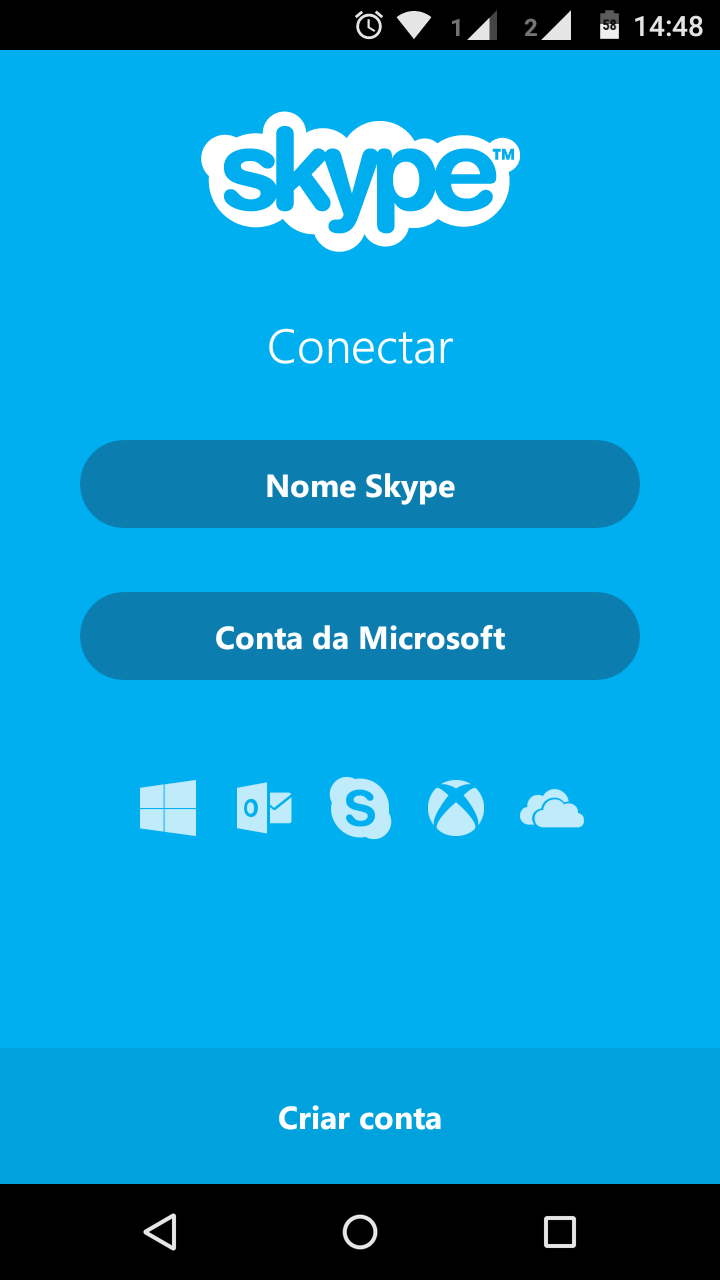
\includegraphics[width=3cm]{figuras/touch/tocar}
    \end{figure}
\end{block}
\end{frame}
%%%%%%%%%%%%%%%%

\begin{frame}{Padrões de Affordance}
\begin{block}{Toque}
    \begin{figure}
    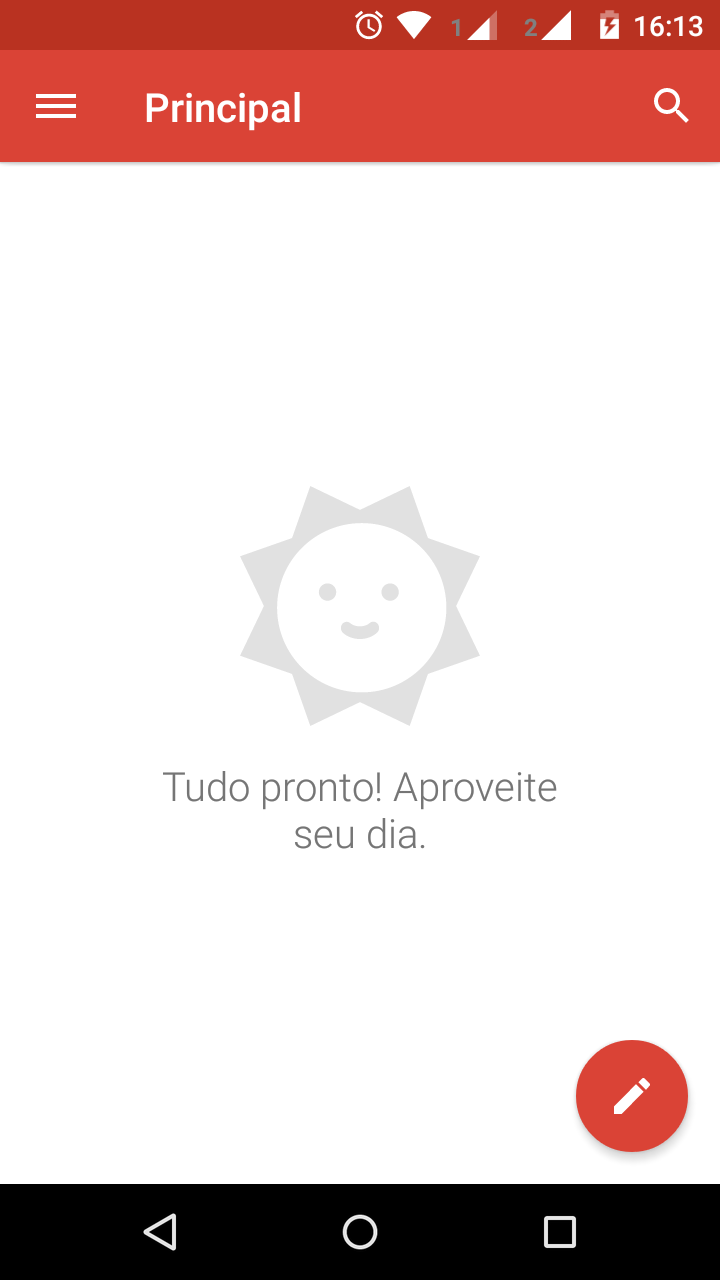
\includegraphics[width=3cm]{figuras/touch/tocar2}
    \end{figure}
\end{block}
\end{frame}
%%%%%%%%%%%%%%%%

\begin{frame}{Padrões de Affordance}
\begin{block}{Deslizar}
  \begin{itemize}
    \item<1-> Essa técnica tem como objetivo indicar ao usuário a possibilidade de que haja mais itens para se ver.
  \end{itemize}
\end{block}
\end{frame}
%%%%%%%%%%%%%%%%

\begin{frame}{Padrões de Affordance}
\begin{block}{Deslizar}
    \begin{figure}
    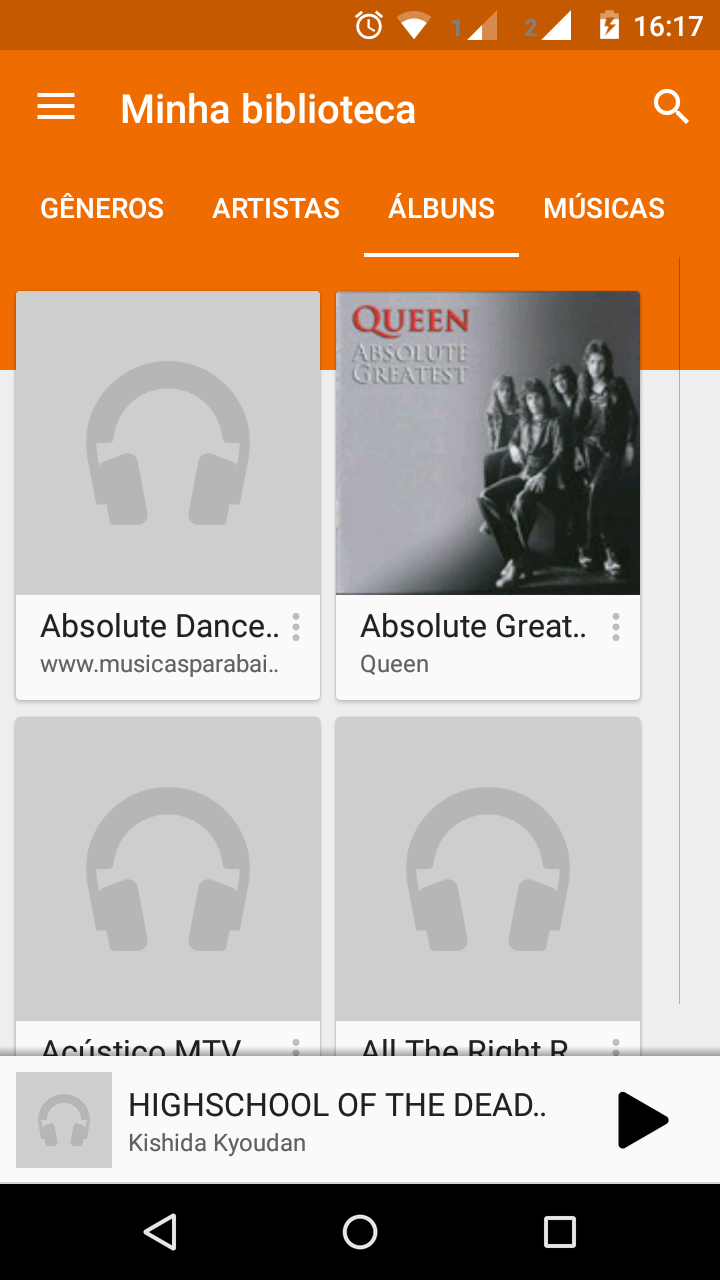
\includegraphics[width=3cm]{figuras/deslize/deslize2}
    \end{figure}
\end{block}
\end{frame}
%%%%%%%%%%%%%%%%

\begin{frame}{Padrões de Affordance}
\begin{block}{Deslizar}
    \begin{figure}
    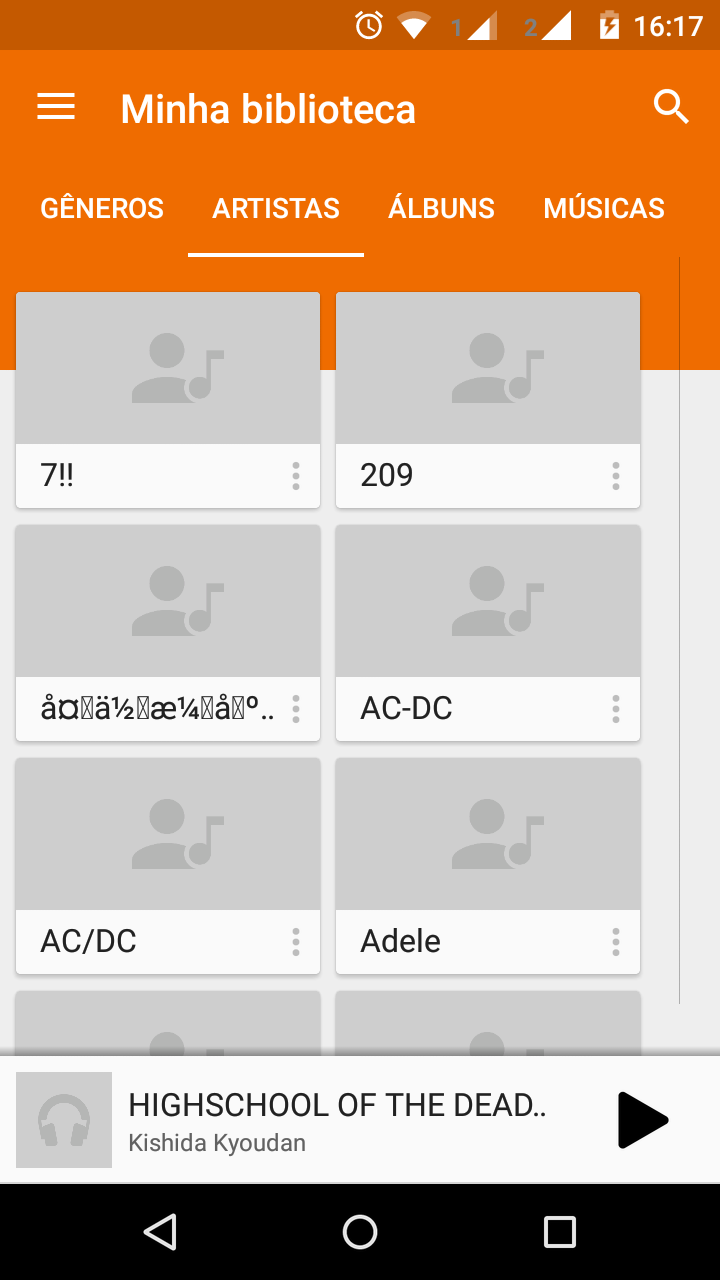
\includegraphics[width=3cm]{figuras/deslize/deslize3}
    \end{figure}
\end{block}
\end{frame}
%%%%%%%%%%%%%%%%

\begin{frame}{Padrões de Affordance}
\begin{block}{Deslizar}
    \begin{figure}
    
\includegraphics[width=3cm]{figuras/deslize/deslize1}
    \end{figure}
\end{block}
\end{frame}
%%%%%%%%%%%%%%%%

\begin{frame}{Padrões de Affordance}
\begin{block}{Deslizar}
    \begin{figure}
    
\includegraphics[width=3cm]{figuras/deslize/deslize6}
    \end{figure}
\end{block}
\end{frame}
%%%%%%%%%%%%%%%%

\begin{frame}{Padrões de Affordance}
\begin{block}{Deslizar}
    \begin{figure}
    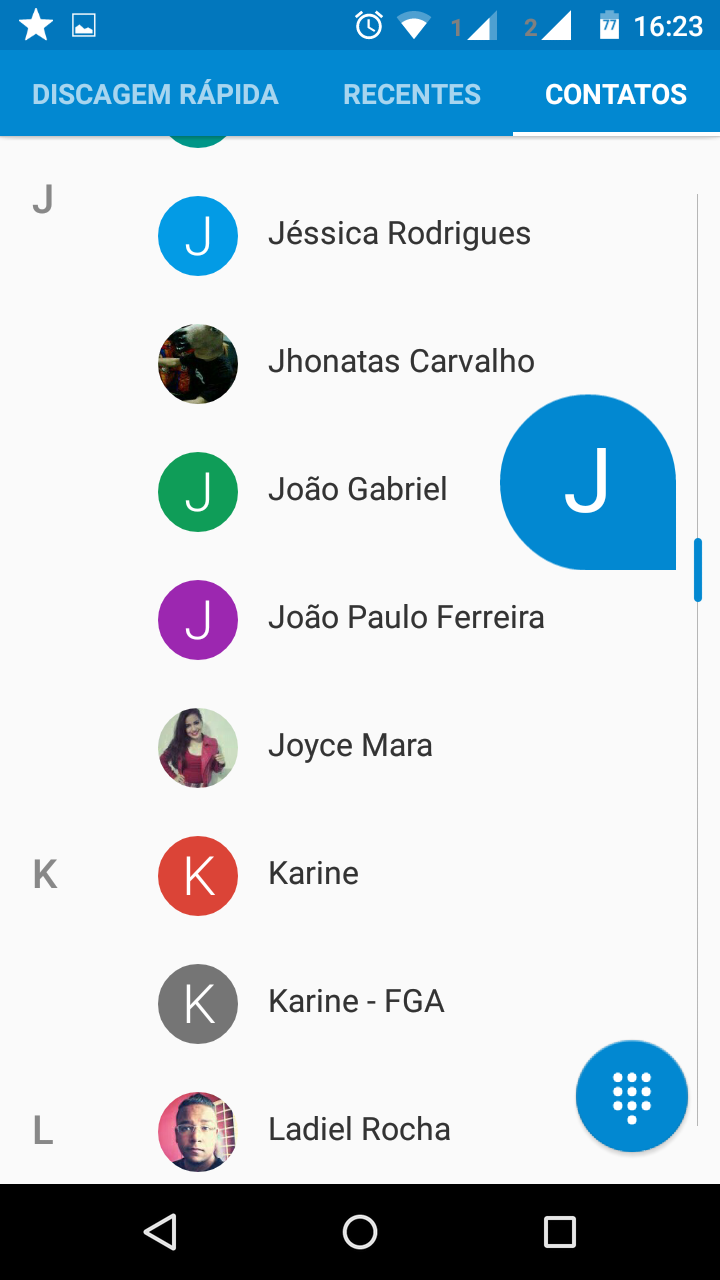
\includegraphics[width=3cm]{figuras/deslize/deslize5}
    \end{figure}
\end{block}
\end{frame}
%%%%%%%%%%%%%%%%

\begin{frame}{Padrões de Affordance}
\begin{block}{Arrastar}
  \begin{itemize}
    \item<1-> Para indicar que determinado item pode ser movido, rearranjado ou reordenado deve se usar o padrão de arrasto.
  \end{itemize}
\end{block}
\end{frame}
%%%%%%%%%%%%%%%%

% ----------------- Referências --------------------------------

% --- O comando \allowframebreaks ---
% Se o conteúdo não se encaixa em um quadro, a opção allowframebreaks instrui
% beamer para quebrá-lo automaticamente entre dois ou mais quadros,
% mantendo o frametitle do primeiro quadro (dado como argumento) e acrescentando
% um número romano ou algo parecido na continuação.

\begin{frame}{Referências}
  \nocite{*}
  \bibliographystyle{plain}
  \bibliography{editaveis/bibliografia}
\end{frame}

% ----------------- FIM DO DOCUMENTO -----------------------------------------

{\aauwavesbg%
\begin{frame}[plain,noframenumbering]%
  \finalpage{Obrigado!}
\end{frame}}
%%%%%%%%%%%%%%%%

\end{document}
